%%%%%%%%%%%%%%%%%%%%%%%%%%ch4-3
\begin{frame}[shrink]
  \frametitle{ch4.信号波形的检测}
  \framesubtitle{ch4-5. 一般二元信号波形的检测---充分统计量的方法}
  \tableofcontents[hideallsubsections]
\end{frame}

\section{一般二元信号波形的检测---充分统计量的方法}

\begin{frame}{一般二元信号波形的检测---充分统计量的方法}
\begin{itemize}
	\setlength{\itemsep}{.5cm}
	\item \textbf{条件: }功率谱密度为$P_n(\omega)=N_0/2$的高斯白噪声背景中一般二元信号波形检测
	\item \textbf{正交级数展开法: }信道噪声是白噪声,正交函数集可任意选取。
	\item \textbf{充分统计量法: }\textcolor{blue}{选取特定的正交函数集},使得有关发送信号的信息只包含在有限的展开系数中。	
\end{itemize}
\end{frame}

\begin{frame}{一般二元信号波形的检测---充分统计量的方法}
信号模型
\begin{align*}
&H_0: x(t)=s_0(t)+n(t), 0\le t\le T\\
&H_1: x(t)=s_1(t)+n(t), 0\le t\le T
\end{align*}
$n(t)$为零均值高斯白噪声
\begin{block}{\textbf{\textcolor{blue}{正交函数集$\{f_k(t)\}$的构造问题}}}
波形相关系数$\rho$:
\[ \rho=\frac{1}{\sqrt{E_{0}E_{1}}}\int_{0}^{T}s_0(t)s_1(t)dt,\quad(|\rho|\le 1) \]
$\rho =0$时, 信号$s_0(t)$与$s_1(t)$正交。\\
$\rho\ne 0$时, 信号$s_0(t)$与$s_1(t)$不正交。	
\end{block}
\end{frame}

\begin{frame}{一般二元信号波形的检测---充分统计量的方法}
$H_0: x(t)=s_0(t)+n(t), 0\le t\le T$\\
$H_1: x(t)=s_1(t)+n(t), 0\le t\le T$\\
\textbf{\textcolor{blue}{(1) 选择一组完备正交函数集,构造两个坐标函数:}}\\
\textbf{第一个坐标函数满足:}\\
\[f_1(t)=\frac{1}{\sqrt{E_1}}s_1(t), \quad E_1=\int_{0}^{T}s_1^2(t)dt\]
$f_1(t)$为确知信号$s_1(t)$的\textbf{归一化函数}。\\
其余坐标函数$f_k(t), k\ge 2$是与$f_1(t)$正交, 且两两正交的任意归一化函数, 即
\[f_j(t)\text{和}f_k(t)\text{是正交的}, k\ge 1, j\ge 1, k\ne j \]
\end{frame}

\begin{frame}[shrink]{格拉姆---施密特正交化法构造$f_2(t)$}
\textbf{格拉姆---施密特(Gram---Schmidt)正交化法构造第二个坐标函数: }\\
~\\
利用$s_0(t)$构造与$f_1(t)$正交的信号$g_2(t)$。
\begin{align*}
g_2(t)&=s_0(t)-s_{01}f_1(t)\\
&=s_0(t)-\left[\int_{0}^{T}s_0(t)f_1(t)dt\right]f_1(t)\\
&=s_0(t)-\left[\int_{0}^{T}s_0(t)\frac{1}{\sqrt{E_1}}s_1(t)dt\right]\frac{1}{\sqrt{E_1}}s_1(t) &&\text{by }f_1(t)=\frac{1}{\sqrt{E_1}}s_1(t)\\
&=s_0(t)-\rho\sqrt{\frac{E_0}{E_1}}s_1(t) &&\text{by }\rho=\frac{1}{\sqrt{E_{0}E_{1}}}\int_{0}^{T}s_0(t)s_1(t)dt\\
\end{align*}
\end{frame}

\begin{frame}[shrink]{格拉姆---施密特法构造$f_2(t)$}
\begin{align*}
&g_2(t)=s_0(t)-\rho\sqrt{\frac{E_0}{E_1}}s_1(t), \int_{0}^{T}s_0^2(t)dt=E_0, \int_{0}^{T}s_1^2(t)dt=E_1, \int_{0}^{T}s_0(t)s_1(t)dt=\rho\sqrt{E_0E_1}
\end{align*}
归一化$g_2(t)$, 得到\textbf{第二个坐标函数:}
\begin{align*}
f_2(t)&=\frac{g_2(t)}{\sqrt{\int_{0}^{T}g_2^2(t)dt}}=\frac{s_0(t)-\rho\sqrt{\frac{E_0}{E_1}}s_1(t)}{\sqrt{\int_{0}^{T}\left(s_0(t)-\rho\sqrt{\frac{E_0}{E_1}}s_1(t)\right)^2dt}}\\
&=\frac{s_0(t)-\rho\sqrt{\frac{E_0}{E_1}}s_1(t)}{\sqrt{\int_{0}^{T}\left(s_0^2(t)-2\rho\sqrt{\frac{E_0}{E_1}}s_0(t)s_1(t)+\rho^2\frac{E_0}{E_1}s_1^2(t)\right)dt}}\\
&=\frac{s_0(t)-\rho\sqrt{\frac{E_0}{E_1}}s_1(t)}{\sqrt{E_0-2\rho\sqrt{\frac{E_0}{E_1}}\rho\sqrt{E_0E_1}+\rho^2\frac{E_0}{E_1}E_1}}
=\frac{1}{\sqrt{(1-\rho^2)E_0}}\left(s_0(t)-\rho\sqrt{\frac{E_0}{E_1}}s_1(t)\right)
\end{align*}
\end{frame}

\begin{frame}[shrink]{证明: $f_1(t)$和$f_2(t)$是正交函数集的前两个坐标函数(1)}
\begin{align*}
&f_1(t)=\frac{1}{\sqrt{E_1}}s_1(t),\quad f_2(t)=\frac{1}{\sqrt{(1-\rho^2)E_0}}\left(s_0(t)-\rho\sqrt{\frac{E_0}{E_1}}s_1(t)\right)\\
&\int_{0}^{T}s_0^2(t)dt=E_0, \int_{0}^{T}s_1^2(t)dt=E_1, \int_{0}^{T}s_0(t)s_1(t)dt=\rho\sqrt{E_0E_1}
\end{align*}
%\begin{proof}
\textbf{证明: } $f_1(t)$和$f_2(t)$满足正交集坐标函数的定义。\\
(1) 先证明$f_1(t), f_2(t)$是\textbf{归一化函数}。因为
\begin{align*}
\int_{0}^{T}f_1^2(t)dt&=\frac{1}{E_1}\int_{0}^{T}s_1^2(t)dt=1\\
\int_{0}^{T}f_2^2(t)dt&=\frac{1}{(1-\rho^2)E_0}\int_{0}^{T}\left(s_0(t)-\rho\sqrt{\frac{E_0}{E_1}}s_1(t)\right)^2dt\\
&=\frac{1}{(1-\rho^2)E_0}\int_{0}^{T}\left(s_0^2(t)-2\rho\sqrt{\frac{E_0}{E_1}}s_0(t)s_1(t)+\rho^2\frac{E_0}{E_1}s_1^2(t)\right)dt\\
&=\frac{1}{(1-\rho^2)E_0}\left(E_0-2\rho\sqrt{\frac{E_0}{E_1}}\rho\sqrt{E_0E_1}+\rho^2\frac{E_0}{E_1}E_1\right)=1
\end{align*}
%\end{proof}
\end{frame}

\begin{frame}[shrink]{证明: $f_1(t)$和$f_2(t)$是正交函数集的前两个坐标函数(2)}
\begin{align*}
&f_1(t)=\frac{1}{\sqrt{E_1}}s_1(t),\quad f_2(t)=\frac{1}{\sqrt{(1-\rho^2)E_0}}\left(s_0(t)-\rho\sqrt{\frac{E_0}{E_1}}s_1(t)\right)\\
&\int_{0}^{T}s_0^2(t)dt=E_0, \int_{0}^{T}s_1^2(t)dt=E_1, \int_{0}^{T}s_0(t)s_1(t)dt=\rho\sqrt{E_0E_1}
\end{align*}
(2) 再证明$f_1(t), f_2(t)$是相互正交的两个函数。因为
\begin{align*}
\int_{0}^{T}f_1(t)f_2(t)dt&=\int_{0}^{T}\frac{1}{\sqrt{E_1}}s_1(t)
\frac{1}{\sqrt{(1-\rho^2)E_0}}\left(s_0(t)-\rho\sqrt{\frac{E_0}{E_1}}s_1(t)\right)dt\\
&=\frac{1}{\sqrt{(1-\rho)^2E_0E_1}}\left(\int_{0}^{T}s_0(t)s_1(t)dt-\rho\sqrt{\frac{E_0}{E_1}}\int_{0}^{T}s_1^2(t)dt\right)\\
&=\frac{1}{\sqrt{(1-\rho)^2E_0E_1}}\left(\rho\sqrt{E_0E_1}-\rho\sqrt{\frac{E_0}{E_1}}E_1\right)=0
\end{align*}
所以, $f_1(t), f_2(t)$是相互正交的两个函数。\\
\textbf{综上(1), (2), $f_1(t), f_2(t)$是归一化函数, 且满足正交性, 是正交函数集的前两个坐标函数。}$\hfill\square$
\end{frame}

\begin{frame}{充分统计量的方法, 选择一组完备正交函数集}
\begin{align*}
&f_1(t)=\frac{1}{\sqrt{E_1}}s_1(t),\quad 0\le t\le T\\
&f_2(t)=\frac{1}{\sqrt{(1-\rho^2)E_0}}\left(s_0(t)-\rho\sqrt{\frac{E_0}{E_1}}s_1(t)\right),\quad 0\le t\le T
\end{align*}
~\\
\vspace{0.2cm}
其余坐标函数$f_k(t), k\ge 3$是与$f_1(t)$和$f_2(t)$正交, 且两两相互正交的任意归一化函数, 即$f_j(t)$和$f_k(t)$是正交的, $k\ge 1, j\ge 1, k\ne j$
\[\int_{0}^{T}f_j(t)f_k(t)dt=0,\quad k\ge 1, j\ge 1, k\ne j\]
\end{frame}

\begin{frame}[shrink]{对接收信号进行正交展开(假设$H_0: x_1$)}
\begin{block}{假设$H_0:x(t)=s_0(t)+n(t)$下,展开系数$x_1$}
\begin{align*}
x_1&=\int_{0}^{T}x(t)f_1(t)dt=\int_{0}^{T}[s_0(t)+n(t)]f_1(t)dt=\int_{0}^{T}s_0(t)f_1(t)dt+\int_{0}^{T}n(t)f_1(t)dt\\
&=\int_{0}^{T}s_0(t)[\frac{1}{\sqrt{E_1}}s_1(t)]dt+n_1=\frac{1}{\sqrt{E_1}}\int_{0}^{T}s_0(t)s_1(t)dt+n_1\\
&=\rho\sqrt{E_0}+n_1
\end{align*}
\end{block}
\begin{align*}
&f_1(t)=\frac{1}{\sqrt{E_1}}s_1(t),\quad \int_{0}^{T}n(t)f_1(t)dt=n_1\\
&\rho=\frac{1}{\sqrt{E_0E_1}}\int_{0}^{T}s_0(t)s_1(t)dt\implies \int_{0}^{T}s_0(t)s_1(t)dt=\rho\sqrt{E_0E_1}
\end{align*}
\end{frame}

\begin{frame}[shrink]{对接收信号进行正交展开(假设$H_0:x_2$)}
\begin{block}{假设$H_0:x(t)=s_0(t)+n(t)$下,展开系数$x_2$}
	\begin{align*}
	x_2&=\int_{0}^{T}x(t)f_2(t)dt=\int_{0}^{T}[s_0(t)+n(t)]f_2(t)dt=\int_{0}^{T}s_0(t)f_2(t)dt+\int_{0}^{T}n(t)f_2(t)dt\\
	&=\int_{0}^{T}s_0(t)\frac{1}{\sqrt{(1-\rho^2)E_0}}\left(s_0(t)-\rho\sqrt{\frac{E_0}{E_1}}s_1(t)\right)dt+n_2\\
	&=\frac{1}{\sqrt{(1-\rho^2)E_0}}\left[\int_{0}^{T}s_0^2(t)dt-\rho\sqrt{\frac{E_0}{E_1}}\int_{0}^{T}s_0(t)s_1(t)dt\right]+n_2\\
	&=\frac{1}{\sqrt{(1-\rho^2)E_0}}\left[E_0-\rho\sqrt{\frac{E_0}{E_1}}\rho\sqrt{E_0E_1}\right]+n_2=\sqrt{(1-\rho^2)E_0}+n_2
	\end{align*}
\end{block}
\begin{align*}
&f_2(t)=\frac{1}{\sqrt{(1-\rho^2)E_0}}\left(s_0(t)-\rho\sqrt{\frac{E_0}{E_1}}s_1(t)\right),\quad E_0=\int_{0}^{T}s_0^2(t)dt,\quad \int_{0}^{T}n(t)f_2(t)dt=n_2\\
&\rho=\frac{1}{\sqrt{E_0E_1}}\int_{0}^{T}s_0(t)s_1(t)dt\implies \int_{0}^{T}s_0(t)s_1(t)dt=\rho\sqrt{E_0E_1}
\end{align*}
\end{frame}

\begin{frame}[shrink]{对接收信号进行正交展开(假设$H_0: x_k$)}
\begin{block}{假设$H_0:x(t)=s_0(t)+n(t)$下,展开系数$x_k$}
	\begin{align*}
	x_k&=\int_{0}^{T}x(t)f_k(t)dt=\int_{0}^{T}[s_0(t)+n(t)]f_k(t)dt=\int_{0}^{T}s_0(t)f_k(t)dt+\int_{0}^{T}n(t)f_k(t)dt\\
	&=0+\int_{0}^{T}n(t)f_k(t)dt=n_k\quad k\ge 3
	\end{align*}
\end{block}
\begin{align*}
&f_2(t)=\frac{1}{\sqrt{(1-\rho^2)E_0}}\left(s_0(t)-\rho\sqrt{\frac{E_0}{E_1}}s_1(t)\right), s_1(t)=\sqrt{E_1}f_1(t)\\
&\implies s_0(t)=\left(\sqrt{(1-\rho^2)E_0}\right)f_2(t)+\left(\rho\sqrt{E_0}\right)f_1(t)\\
&\int_{0}^{T}f_j(t)f_k(t)dt=0,\quad k\ge 1, j\ge 1, k\ne j
\end{align*}
\end{frame}

\begin{frame}[shrink]{对接收信号进行正交展开(假设$H_1$)}
\begin{block}{假设$H_1:x(t)=s_1(t)+n(t)$下,展开系数}
\begin{align*}
	x_1&=\int_{0}^{T}x(t)f_1(t)dt=\int_{0}^{T}[s_1(t)+n(t)]f_1(t)dt=\int_{0}^{T}s_1(t)f_1(t)dt+\int_{0}^{T}n(t)f_1(t)dt\\
	&=\int_{0}^{T}s_1(t)[\frac{1}{\sqrt{E_1}}s_1(t)]dt+n_1=\frac{1}{\sqrt{E_1}}\int_{0}^{T}s_1^2(t)dt+n_1\\
	&=\sqrt{E_1}+n_1\quad (\text{by }f_1(t)=\frac{1}{\sqrt{E_1}}s_1(t),E_1=\int_{0}^{T}s_1^2(t)dt)\\
	x_2&=\int_{0}^{T}x(t)f_2(t)dt=\int_{0}^{T}[s_1(t)+n(t)]f_2(t)dt=\int_{0}^{T}s_1(t)f_2(t)dt+\int_{0}^{T}n(t)f_2(t)dt\\
	&=\int_{0}^{T}[\sqrt{E_1}f_1(t)]f_2(t)dt+n_2=0+n_2=n_2\\
	x_k&=\int_{0}^{T}x(t)f_k(t)dt=\int_{0}^{T}[s_1(t)+n(t)]f_k(t)dt=\int_{0}^{T}[\sqrt{E_1}f_1(t)+n(t)]f_k(t)dt\\
	&=\int_{0}^{T}n(t)f_k(t)dt=n_k\quad k\ge 3\quad (by\quad s_1(t)=\sqrt{E_1}f_1(t), \int_{0}^{T}f_1(t)f_k(t)dt=0,k\ge 3)
\end{align*}
\end{block}
\end{frame}

\begin{frame}[shrink]{充分量统计法}
\textbf{\textcolor{blue}{(2)利用构造的正交函数集$f_1(t),f_2(t)$和$\{f_k(t)|k\ge 3\}$对接收信号进行正交展开}}
\begin{block}{两个假设下展开系数$x_1,x_2$}
\begin{align*}
&x_1|H_0=\int_{0}^{T}x(t)f_1(t)dt=\int_{0}^{T}[s_0(t)+n(t)]f_1(t)dt=\rho\sqrt{E_0}+n_1\\
&x_2|H_0=\int_{0}^{T}x(t)f_2(t)dt=\int_{0}^{T}[s_0(t)+n(t)]f_2(t)dt=\sqrt{(1-\rho^2)E_0}+n_2\\
&x_1|H_1=\int_{0}^{T}x(t)f_1(t)dt=\int_{0}^{T}[s_1(t)+n(t)]f_1(t)dt=\sqrt{E_1}+n_1\\
&x_2|H_1=\int_{0}^{T}x(t)f_2(t)dt=\int_{0}^{T}[s_1(t)+n(t)]f_2(t)dt=n_2\\
&H_0,H_1: x_k=\int_{0}^{T}x(t)f_k(t)dt=n_k \quad (k\ge 3)\implies\text{不含确知信号$s_0(t),s_1(t)$信息}
\end{align*}
\end{block}
\textbf{\textcolor{blue}{$\bm{x}=(x_1,x_2)^T$是充分统计量。且$x_1$和$x_2$为高斯随机变量, 相互统计独立。}}
\end{frame}

\begin{frame}[shrink]{充分量统计法: $x_1,x_2$的均值和方差}
\begin{align*}
&E[x_1|H_0]=E\left[\rho\sqrt{E_0}+n_1\right]=\rho\sqrt{E_0}\\
&E[x_2|H_0]=E\left[\sqrt{(1-\rho^2)E_0}+n_2\right]=\sqrt{(1-\rho^2)E_0}\\
&Var[x_1|H_0]=Var[x_2|H_0]=E[n_1^2]=E[n_2^2]=\frac{N_0}{2}\\
&E[x_1|H_1]=E\left[\sqrt{E_1}+n_1\right]=\sqrt{E_1}\\
&E[x_2|H_1]=E[n_2]=0\\
&Var[x_1|H_1]=Var[x_2|H_1]=E[n_1^2]=E[n_2^2]=\frac{N_0}{2}\\
\end{align*}
\end{frame}

\begin{frame}[shrink]{充分量统计法---构建似然比}
\textbf{\textcolor{blue}{(3)利用得到的展开系数,构建似然比表达式
}}
\begin{align*}
\bm{x}=(x_1,x_2)^T\\
\lambda(\bm{x})=\frac{p(\bm{x}|H_1)}{p(\bm{x}|H_0)}\mathop{\gtrless}_{H_0}^{H_1}\eta\\
\lambda(\bm{x})=\frac{p(x_1,x_2|H_1)}{p(x_1,x_2|H_0)}\mathop{\gtrless}_{H_0}^{H_1}\eta\\
\frac{\frac{1}{\sqrt{\pi N_0}}\exp\left(-\frac{\left(x_1-\sqrt{E_1}\right)^2}{N_0}\right)\frac{1}{\sqrt{\pi N_0}}\exp\left(-\frac{x_2^2}{N_0}\right)}
{\frac{1}{\sqrt{\pi N_0}}\exp\left(-\frac{\left(x_1-\rho\sqrt{E_0}\right)^2}{N_0}\right)\frac{1}{\sqrt{\pi N_0}}\exp\left(-\frac{\left(x_2-\sqrt{(1-\rho^2)E_0}\right)^2}{N_0}\right)}
\mathop{\gtrless}_{H_0}^{H_1}\eta
\end{align*}
\end{frame}

\begin{frame}[shrink]{充分量统计法---构建似然比}
\textbf{\textcolor{blue}{(3)利用得到的展开系数,构建似然比表达式
}}\\
取对数化简
\begin{align*}
&\exp\left(
\frac{1}{N_0}\left[\left(x_1-\rho\sqrt{E_0}\right)^2+
\left(x_2-\sqrt{(1-\rho^2)E_0}\right)^2\right]-
\frac{1}{N_0}\left[\left(x_1-\sqrt{E_1}\right)^2+x_2^2\right]
\right)\mathop{\gtrless}_{H_0}^{H_1}\eta\\
&\frac{1}{N_0}\left[
2\sqrt{E_1}x_1-2\rho\sqrt{E_0}x_1-2\sqrt{(1-\rho^2)E_0}x_2-E_1+E_0
\right]\mathop{\gtrless}_{H_0}^{H_1}\ln\eta\\
&\left(\sqrt{E_1}-\rho\sqrt{E_0}\right)x_1-\left(\sqrt{(1-\rho^2)E_0}\right)x_2\mathop{\gtrless}_{H_0}^{H_1}\frac{N_0}{2}\ln\eta+\frac{1}{2}(E_1-E_0)\\
\end{align*}
检验统计量:
\begin{align*}
l[x(t)]&=\left(\sqrt{E_1}-\rho\sqrt{E_0}\right)x_1-\left(\sqrt{(1-\rho^2)E_0}\right)x_2\\
&=\left(\sqrt{E_1}-\rho\sqrt{E_0}\right)\int_{0}^{T}x(t)f_1(t)dt-\left(\sqrt{(1-\rho^2)E_0}\right)\int_{0}^{T}x(t)f_2(t)dt\\
\end{align*}
\end{frame}

\begin{frame}[shrink]{充分量统计法---构建似然比}
\textbf{\textcolor{blue}{(3)利用得到的展开系数,构建似然比表达式
}}\\
检验统计量:
\begin{align*}
l[x(t)]&=\left(\sqrt{E_1}-\rho\sqrt{E_0}\right)\int_{0}^{T}x(t)f_1(t)dt-\left(\sqrt{(1-\rho^2)E_0}\right)\int_{0}^{T}x(t)f_2(t)dt\\
&=\left(\sqrt{E_1}-\rho\sqrt{E_0}\right)\int_{0}^{T}x(t)\frac{1}{\sqrt{E_1}}s_1(t)dt\\
&- \left(\sqrt{(1-\rho^2)E_0}\right)\int_{0}^{T}x(t)\frac{1}{\sqrt{(1-\rho^2)E_0}}\left(s_0(t)-\rho\sqrt{\frac{E_0}{E_1}}s_1(t)\right)dt\\
&=\left(1-\rho\sqrt{\frac{E_0}{E_1}}\right)\int_{0}^{T}x(t)s_1(t)dt-\int_{0}^{T}x(t)\left(s_0(t)-\rho\sqrt{\frac{E_0}{E_1}}s_1(t)\right)dt\\
&=\int_{0}^{T}x(t)s_1(t)dt-\int_{0}^{T}x(t)s_0(t)dt
\end{align*}
\end{frame}

\begin{frame}[shrink]{充分量统计法---判决表达式}
\begin{align*}
l[x(t)]\mathop{=}^{def}\int_{0}^{T}x(t)s_1(t)dt-\int_{0}^{T}x(t)s_0(t)dt\mathop{\gtrless}_{H_0}^{H_1}\frac{N_0}{2}\ln\eta+\frac{1}{2}(E_1-E_0)\mathop{=}^{def}\gamma
\end{align*}
\begin{block}{结论}
	由任意正交函数集对$x(t)$进行正交级数展开法与由充分统计量法导出的判决表达式是完全一样的,因而也具有相同的检测系统结构和相同的检测性能。
\end{block}
\end{frame}

\begin{frame}{一般二元信号波形的检测例题1}
考虑发送信号周期为$T=2\pi/\omega_0$的二元移频键控系统。在假设$H_0$和$H_1$下的发送信号分别为:
\begin{align*}
&H_0: x(t)=a\sin\omega_0t+n(t), \quad 0\le t\le T\\
&H_1: x(t)=a\sin2\omega_0t+n(t), \quad 0\le t\le T
\end{align*}
其中, 信号的振幅$a$和频率$\omega_0$已知, 并假定两个假设先验等概。信号在传输中叠加了均值为零, 功率谱密度为$N_0/2$的高斯白噪声$n(t)$。\\
~\\
现采用最小平均错误概率准则, 设计信号检测系统, 并计算平均错误概率$P_e$。
\end{frame}

\begin{frame}{一般二元信号波形的检测例题1: 解}
解: 根据题设, 得到两个确知信号的能量分别为
\begin{align*}
E_0&=\int_{0}^{T}s_0^2(t)dt=\int_{0}^{T}(a\sin\omega_0t)^2dt=\frac{a^2T}{2}\\
E_1&=\int_{0}^{T}s_1^2(t)dt=\int_{0}^{T}(a\sin2\omega_0t)^2dt=\frac{a^2T}{2}\\
E_s&\mathop{=}^{def}E_0=E_1=\frac{a^2T}{2}
\end{align*}
由于两个假设的先验概率等概, 因此在最小平均错误概率准则下, 判决门限$\eta=1$, 利用一般二元信号检测波形判决表达式, 得
\begin{align*}
l[x(t)]\mathop{=}^{def}\int_{0}^{T}x(t)s_1(t)dt-\int_{0}^{T}x(t)s_0(t)dt&\mathop{\gtrless}_{H_0}^{H_1}\frac{N_0}{2}\ln\eta+\frac{1}{2}(E_1-E_0)=0\\
\int_{0}^{T}x(t)a\sin2\omega_0tdt-\int_{0}^{T}x(t)a\sin\omega_0tdt&\mathop{\gtrless}_{H_0}^{H_1}0
\end{align*}
\end{frame}

\begin{frame}[shrink]{一般二元信号波形的检测例题1: 解(续1)}
为求平均错误概率, 首先需要计算偏移系数$d^2$
\[d^2\mathop{=}\limits^{def}\frac{\left(E[l|H_1]-E[l|H_0]\right)^2}{Var[l|H_0]}\]
\[
l[x(t)]=\int_{0}^{T}x(t)a\sin2\omega_0tdt-\int_{0}^{T}x(t)a\sin\omega_0tdt \]
\begin{align*}
E[l|H_0]&=E\left[\int_{0}^{T}x(t)a\sin2\omega_0tdt-\int_{0}^{T}x(t)a\sin\omega_0tdt|H_0\right]\quad \text{by } x(t)=a\sin\omega_0t+n(t)\\
&=E\left[\int_{0}^{T}[a\sin\omega_0t+n(t)]a\sin2\omega_0tdt-\int_{0}^{T}[a\sin\omega_0t+n(t)]a\sin\omega_0tdt\right]\\
&=E\left[a^2\int_{0}^{T}\sin\omega_0t\sin2\omega_0tdt\right]+\int_{0}^{T}E[n(t)]a\sin2\omega_0tdt\\
&\quad -E\left[\int_{0}^{T}(a\sin\omega_0t)^2dt\right]-\int_{0}^{T}E[n(t)]a\sin\omega_0tdt\quad\text{by }E[n(t)]=0\\
&=0+0-E\left[\int_{0}^{T}(a\sin\omega_0t)^2dt\right]-0=-E_0=-E_s
\end{align*}
\end{frame}

\begin{frame}[shrink]{一般二元信号波形的检测例题1: 解(续2)}
\begin{align*}
&H_0: x(t)=a\sin\omega_0t+n(t),\quad E[l|H_0]=-E_s\\
&Var[l|H_0]=E\left[\left((l|H_0)-E[l|H_0]\right)^2\right]\\
&=E\left[\left(\int_{0}^{T}x(t)a\sin2\omega_0tdt-\int_{0}^{T}x(t)a\sin\omega_0tdt|H_0+E_s\right)^2\right]\\
&=E\left[\left(\int_{0}^{T}[a\sin\omega_0t+n(t)]a\sin2\omega_0tdt-\int_{0}^{T}[a\sin\omega_0t+n(t)]a\sin\omega_0tdt+E_s\right)^2\right]\\
&=E\left[\left(0+\int_{0}^{T}n(t)a\sin2\omega_0tdt-E_0-\int_{0}^{T}n(t)a\sin\omega_0tdt+E_s\right)^2\right]\\
&=E\left[\left(\int_{0}^{T}n(t)a\sin2\omega_0tdt-\int_{0}^{T}n(t)a\sin\omega_0tdt\right)^2\right]\\
&=E\left[\left(\int_{0}^{T}n(t)a\sin2\omega_0tdt\right)^2\right]+E\left[\left(\int_{0}^{T}n(t)a\sin\omega_0tdt\right)^2\right]\\
&\quad -2E\left[\int_{0}^{T}n(t)a\sin2\omega_0tdt\int_{0}^{T}n(u)a\sin\omega_0udu\right]
\end{align*}
\end{frame}

\begin{frame}[shrink]{一般二元信号波形的检测例题1: 解(续3)}
\begin{align*}
&E\left[\left(\int_{0}^{T}n(t)a\sin2\omega_0tdt\right)^2\right]=E\left[\int_{0}^{T}n(t)a\sin2\omega_0tdt\int_{0}^{T}n(u)a\sin2\omega_0udu\right]\\
&=\int_{0}^{T}a\sin2\omega_0t\left[\int_{0}^{T}E[n(t)n(u)]a\sin2\omega_0udu\right]dt\quad\text{by }E[n(t)n(u)]=\frac{N_0}{2}\delta(t-u)\\
&=\int_{0}^{T}a\sin2\omega_0t\left[\int_{0}^{T}\frac{N_0}{2}\delta(t-u)a\sin2\omega_0udu\right]dt\quad\text{by $\delta$的筛选性}\\
&=\int_{0}^{T}a\sin2\omega_0t\left[\frac{N_0}{2}a\sin2\omega_0t\right]dt=\frac{N_0}{2}\int_{0}^{T}(a\sin2\omega_0t)^2dt=\frac{N_0E_1}{2}\\
&\text{类似地有, }\quad E\left[\left(\int_{0}^{T}n(t)a\sin\omega_0tdt\right)^2\right]=\frac{N_0E_0}{2}\\
&E\left[\int_{0}^{T}n(t)a\sin2\omega_0tdt\int_{0}^{T}n(u)a\sin\omega_0udu\right]\\
&=\int_{0}^{T}a\sin2\omega_0t\left[\int_{0}^{T}E[n(t)n(u)]a\sin\omega_0udu\right]dt\\
&=\frac{a^2N_0}{2}\int_{0}^{T}\sin2\omega_0t\sin\omega_0tdt=0
\end{align*}
\end{frame}

\begin{frame}[shrink]{一般二元信号波形的检测例题1: 解(续4)}
\begin{align*}
Var[l|H_0]&=E\left[\left(\int_{0}^{T}n(t)a\sin2\omega_0tdt\right)^2\right]+E\left[\left(\int_{0}^{T}n(t)a\sin\omega_0tdt\right)^2\right]\\
&\quad -2E\left[\int_{0}^{T}n(t)a\sin2\omega_0tdt\int_{0}^{T}n(u)a\sin2\omega_0udu\right]\\
&=\frac{N_0E_1}{2}+\frac{N_0E_0}{2}-0\\
&=N_0E_s
\end{align*}
\end{frame}

\begin{frame}[shrink]{一般二元信号波形的检测例题1: 解(续5)}
\begin{align*}
&E[l|H_1]=E\left[\int_{0}^{T}x(t)a\sin2\omega_0tdt-\int_{0}^{T}x(t)a\sin\omega_0tdt|H_1\right]\quad \text{by } x(t)=a\sin2\omega_0t+n(t)\\
&=E\left[\int_{0}^{T}[a\sin2\omega_0t+n(t)]a\sin2\omega_0tdt-\int_{0}^{T}[a\sin2\omega_0t+n(t)]a\sin\omega_0tdt\right]\\
&=E\left[\int_{0}^{T}(a\sin2\omega_0t)^2dt\right]+\int_{0}^{T}E[n(t)]a\sin2\omega_0tdt\\
&\quad -E\left[a^2\int_{0}^{T}\sin2\omega_0t\sin\omega_0tdt\right]-\int_{0}^{T}E[n(t)]a\sin\omega_0tdt\quad\text{by }E[n(t)]=0\\
&=E\left[\int_{0}^{T}(a\sin2\omega_0t)^2dt\right]+0-0-0=E_1=E_s\\
&Var[l|H_1]=Var[l|H_0]=N_0E_s
\end{align*}
\end{frame}

\begin{frame}[shrink]{一般二元信号波形的检测例题1: 解(续6)}
\[
d^2\mathop{=}^{def}\frac{\left(E[l|H_1]-E[l|H_0]\right)^2}{Var[l|H_0]}=\frac{\left(E_s-(-E_s)\right)^2}{N_0E_s}=\frac{4E_s}{N_0}
\]
判决概率为
\begin{align*}
P(H_1|H_0)&\mathop{=}^{def}P_F=\int_{\gamma}^{\infty}p(l|H_0)dl=Q\left(\frac{\ln\eta}{d}+\frac{d}{2}\right)=Q\left(\frac{d}{2}\right)=Q\left(\sqrt{\frac{E_s}{N_0}}\right)\\
P(H_1|H_1)&\mathop{=}^{def}P_D=\int_{\gamma}^{\infty}p(l|H_1)dl=Q\left(\frac{\ln\eta}{d}-\frac{d}{2}\right)=Q\left(-\sqrt{\frac{E_s}{N_0}}\right)\\
P(H_0|H_1)&=1-P(H_1|H_1)=1-Q\left(-\sqrt{\frac{E_s}{N_0}}\right)=Q\left(\sqrt{\frac{E_s}{N_0}}\right)\\
P_e&=P(H_0)P(H_1|H_0)+P(H_1)P(H_0|H_1)\\
&=\frac{1}{2}P(H_1|H_0)+\frac{1}{2}P(H_0|H_1)\\
&=Q\left(\sqrt{\frac{E_s}{N_0}}\right)
\end{align*}
\end{frame}

\begin{frame}{一般二元信号波形的检测例题2}
设连续相位移频键控通信系统, 在假设$H_0$和$H_1$下的发送信号分别为:
\begin{align*}
&H_0: x(t)=a\sin\omega_0t+n(t), \quad 0\le t\le T\\
&H_1: x(t)=a\sin\omega_1t+n(t), \quad 0\le t\le T
\end{align*}
其中, 信号的振幅$a$和频率$\omega_0, \omega_1$已知, 并假定两个假设先验等概。信号在传输中叠加了均值为零, 功率谱密度为$N_0/2$的高斯白噪声$n(t)$。\\
~\\
问使最小平均错误概率$P_e$最小的两个信号的差频$\omega_d=\omega_1-\omega_0$为多少?
\end{frame}

\begin{frame}{一般二元信号波形的检测例题2: 解}
解: 根据题设, 得到两个确知信号的能量分别为
\begin{align*}
E_0&=\int_{0}^{T}s_0^2(t)dt=\int_{0}^{T}(a\sin\omega_0t)^2dt=\frac{a^2T}{2}\\
E_1&=\int_{0}^{T}s_1^2(t)dt=\int_{0}^{T}(a\sin\omega_1t)^2dt=\frac{a^2T}{2}\\
E_s&\mathop{=}^{def}E_0=E_1=\frac{a^2T}{2}
\end{align*}
由于两个假设的先验概率等概, 因此在最小平均错误概率准则下, 判决门限$\eta=1$, 利用一般二元信号检测波形判决表达式, 得
\begin{align*}
l[x(t)]\mathop{=}^{def}\int_{0}^{T}x(t)s_1(t)dt-\int_{0}^{T}x(t)s_0(t)dt&\mathop{\gtrless}_{H_0}^{H_1}\frac{N_0}{2}\ln\eta+\frac{1}{2}(E_1-E_0)=0\\
\int_{0}^{T}x(t)a\sin\omega_1tdt-\int_{0}^{T}x(t)a\sin\omega_0tdt&\mathop{\gtrless}_{H_0}^{H_1}0
\end{align*}
\end{frame}

\begin{frame}[shrink]{一般二元信号波形的检测例题2: 解(续1)}
为求平均错误概率, 首先需要计算偏移系数$d^2$
\[d^2\mathop{=}\limits^{def}\frac{\left(E[l|H_1]-E[l|H_0]\right)^2}{Var[l|H_0]}\]
\[
l[x(t)]=\int_{0}^{T}x(t)s_1(t)dt-\int_{0}^{T}x(t)s_0(t)dt \]
\begin{align*}
E[l|H_0]&=E\left[\int_{0}^{T}x(t)s_1(t)dt-\int_{0}^{T}x(t)s_0(t)|H_0\right]\quad \text{by } x(t)=s_0(t)+n(t)\\
&=E\left[\int_{0}^{T}[s_0(t)+n(t)]s_1(t)dt-\int_{0}^{T}[s_0(t)+n(t)]s_0(t)dt\right]\\
&=E\left[\int_{0}^{T}s_0(t)s_1(t)dt\right]+\int_{0}^{T}E[n(t)]s_1(t)dt-E\left[\int_{0}^{T}s_0^2(t)dt\right]-\int_{0}^{T}E[n(t)]s_0(t)dt\quad\text{by }E[n(t)]=0\\
&=E\left[\int_{0}^{T}s_0(t)s_1(t)dt\right]-E\left[\int_{0}^{T}s_0^2(t)dt\right]\quad\text{by }E_0=\int_{0}^{T}s_0^2(t)dt\\
&=\rho\sqrt{E_0E_1}-E_0=\rho E_s-E_s\quad\text{by }E_0=E_1=E_s\\
&\text{相关系数}\quad \rho=\frac{1}{\sqrt{E_{0}E_{1}}}\int_{0}^{T}s_0(t)s_1(t)dt=\frac{1}{E_s}\int_{0}^{T}s_0(t)s_1(t)dt,\quad(|\rho|\le 1)
\end{align*}
\end{frame}

\begin{frame}[shrink]{一般二元信号波形的检测例题2: 解(续2)}
\begin{align*}
&H_0: x(t)=a\sin\omega_0t+n(t),\quad E[l|H_0]=\rho E_s-E_s\\
&\rho=\frac{1}{\sqrt{E_{0}E_{1}}}\int_{0}^{T}s_0(t)s_1(t)dt=\frac{1}{E_s}\int_{0}^{T}s_0(t)s_1(t)dt,\quad(|\rho|\le 1)\\
&Var[l|H_0]=E\left[\left((l|H_0)-E[l|H_0]\right)^2\right]\\
&=E\left[\left(\int_{0}^{T}x(t)s_1(t)dt-\int_{0}^{T}x(t)s_0(t)dt|H_0-\rho E_s+E_s\right)^2\right]\\
&=E\left[\left(\int_{0}^{T}[s_0(t)+n(t)]s_1(t)dt-\int_{0}^{T}[s_0(t)+n(t)]s_0(t)dt-\rho E_s+E_s\right)^2\right]\\
&=E\left[\left(\int_{0}^{T}s_0(t)s_1(t)dt+\int_{0}^{T}n(t)s_1(t)dt-\int_{0}^{T}s_0^2(t)dt-\int_{0}^{T}n(t)s_0(t)dt-\rho E_s+E_s\right)^2\right]\\
&=E\left[\left(\rho E_s+\int_{0}^{T}n(t)s_1(t)dt-E_0-\int_{0}^{T}n(t)s_0(t)dt-\rho E_s+E_s\right)^2\right]
=E\left[\left(\int_{0}^{T}n(t)s_1(t)dt-\int_{0}^{T}n(t)s_0(t)dt\right)^2\right]\\
&=E\left[\left(\int_{0}^{T}n(t)s_1(t)dt\right)^2\right]+E\left[\left(\int_{0}^{T}n(t)s_0(t)dt\right)^2\right]-2E\left[\int_{0}^{T}n(t)s_1(t)dt\int_{0}^{T}n(u)s_0(t)du\right]
\end{align*}
\end{frame}

\begin{frame}[shrink]{一般二元信号波形的检测例题2: 解(续3)}
\begin{align*}
&E\left[\left(\int_{0}^{T}n(t)s_1(t)dt\right)^2\right]=E\left[\int_{0}^{T}n(t)s_1(t)dt\int_{0}^{T}n(u)s_1(u)du\right]\\
&=\int_{0}^{T}s_1(t)\left[\int_{0}^{T}E[n(t)n(u)]s_1(u)du\right]dt\quad\text{by }E[n(t)n(u)]=\frac{N_0}{2}\delta(t-u)\\
&=\int_{0}^{T}s_1(t)\left[\int_{0}^{T}\frac{N_0}{2}\delta(t-u)s_1(u)du\right]dt\quad\text{by $\delta$的筛选性}\\
&=\int_{0}^{T}s_1(t)\left[\frac{N_0}{2}s_1(t)\right]dt=\frac{N_0}{2}\int_{0}^{T}s_1^2(t)dt=\frac{N_0E_1}{2}\\
&\text{类似地有, }\quad E\left[\left(\int_{0}^{T}n(t)s_0(t)dt\right)^2\right]=\frac{N_0E_0}{2}\\
&E\left[\int_{0}^{T}n(t)s_1(t)dt\int_{0}^{T}n(u)s_0(u)du\right]
=\int_{0}^{T}s_1(t)\left[\int_{0}^{T}E[n(t)n(u)]s_0(u)du\right]dt\\
&=\frac{N_0}{2}\int_{0}^{T}s_1(t)s_0(t)dt=\frac{N_0\rho E_s}{2}
\end{align*}
\end{frame}

\begin{frame}[shrink]{一般二元信号波形的检测例题2: 解(续4)}
\begin{align*}
Var[l|H_0]&=E\left[\left(\int_{0}^{T}n(t)s_1(t)dt\right)^2\right]+E\left[\left(\int_{0}^{T}n(t)s_0(t)dt\right)^2\right] -2E\left[\int_{0}^{T}n(t)s_1(t)dt\int_{0}^{T}n(u)s_0(t)du\right]\\
&=\frac{N_0E_1}{2}+\frac{N_0E_0}{2}-N_0\rho E_s=\frac{N_0}{2}(E_s+E_s-2\rho E_s)=N_0E_s(1-\rho)\\
E[l|H_1]&=E\left[\int_{0}^{T}x(t)s_1(t)dt-\int_{0}^{T}x(t)s_0(t)|H_1\right]\quad \text{by } x(t)=s_1(t)+n(t)\\
&=E\left[\int_{0}^{T}[s_1(t)+n(t)]s_1(t)dt-\int_{0}^{T}[s_1(t)+n(t)]s_0(t)dt\right]\\
&=E\left[\int_{0}^{T}s_1^2(t)dt\right]+\int_{0}^{T}E[n(t)]s_1(t)dt-E\left[\int_{0}^{T}s_1(t)s_0(t)dt\right]-\int_{0}^{T}E[n(t)]s_0(t)dt\\
&=E\left[\int_{0}^{T}s_1^2(t)dt\right]-E\left[\int_{0}^{T}s_1(t)s_0(t)dt\right]\quad\text{by }E_1=\int_{0}^{T}s_1^2(t)dt\\
&=E_1-\rho\sqrt{E_0E_1}=E_s-\rho E_s\quad\text{by }E_0=E_1=E_s\\
&\text{相关系数}\quad \rho=\frac{1}{\sqrt{E_{0}E_{1}}}\int_{0}^{T}s_0(t)s_1(t)dt=\frac{1}{E_s}\int_{0}^{T}s_0(t)s_1(t)dt,\quad(|\rho|\le 1)
\end{align*}
\end{frame}

\begin{frame}[shrink]{一般二元信号波形的检测例题2: 解(续5)}
\[
d^2\mathop{=}^{def}\frac{\left(E[l|H_1]-E[l|H_0]\right)^2}{Var[l|H_0]}=\frac{\left(E_s-\rho E_s-(\rho E_s-E_s)\right)^2}{N_0E_s(1-\rho)}=\frac{4E_s}{N_0}(1-\rho)
\]
判决概率为
\begin{align*}
P(H_1|H_0)&\mathop{=}^{def}P_F=\int_{\gamma}^{\infty}p(l|H_0)dl=Q\left[\frac{\ln\eta}{d}+\frac{d}{2}\right]=Q\left[\frac{d}{2}\right]=Q\left[\sqrt{\frac{E_s}{N_0}(1-\rho)}\right]\\
P(H_1|H_1)&\mathop{=}^{def}P_D=\int_{\gamma}^{\infty}p(l|H_1)dl=Q\left[\frac{\ln\eta}{d}-\frac{d}{2}\right]=Q\left[-\sqrt{\frac{E_s}{N_0}(1-\rho)}\right]\\
P(H_0|H_1)&=1-P(H_1|H_1)=1-Q\left[-\sqrt{\frac{E_s}{N_0}(1-\rho)}\right]=Q\left[\sqrt{\frac{E_s}{N_0}(1-\rho)}\right]\\
P_e&=P(H_0)P(H_1|H_0)+P(H_1)P(H_0|H_1)\\
&=\frac{1}{2}P(H_1|H_0)+\frac{1}{2}P(H_0|H_1)\\
&=Q\left[\sqrt{\frac{E_s}{N_0}(1-\rho)}\right]
\end{align*}
\end{frame}

\begin{frame}[shrink]{一般二元信号波形的检测例题2: 解(续6)}
\begin{align*}
P_e=Q\left[\sqrt{\frac{E_s}{N_0}(1-\rho)}\right]
\end{align*}
由上式可知, 为使平均错误概率最小,需使$\frac{E_s}{N_0}(1-\rho)$取得最小值, 又由于
\begin{align*}
\rho&=\frac{1}{\sqrt{E_{0}E_{1}}}\int_{0}^{T}s_0(t)s_1(t)dt=\frac{1}{E_s}\int_{0}^{T}s_0(t)s_1(t)dt\\
&=\frac{a^2}{E_s}\int_{0}^{T}\sin\omega_1t\sin\omega_0tdt\quad\text{by }E_s=\frac{a^2T}{2}\\
&=\frac{2}{T}\int_{0}^{T}\sin\omega_1t\sin\omega_0tdt\\
&=\frac{1}{T}\int_{0}^{T}\cos(\omega_1-\omega_0)tdt-\frac{1}{T}\int_{0}^{T}\cos(\omega_1+\omega_0)tdt\\
&=\left.\frac{1}{T}\cdot\frac{1}{\omega_1-\omega_0}\sin(\omega_1-\omega_0)t\right|_0^T=\frac{\sin\omega_dT}{\omega_dT}
\end{align*}
\end{frame}

\begin{frame}[shrink]{一般二元信号波形的检测例题2: 解(续7)}
\begin{align*}
\rho=\frac{\sin\omega_dT}{\omega_dT}
\end{align*}
由上式可知, 相关系数与频率差有关, 令
\begin{align*}
\frac{\partial\rho}{\partial\omega_d}=\frac{1}{T}\cdot\frac{(\cos\omega_dT)\omega_dT-\sin\omega_dT}{\omega_d^2}=0
\end{align*}
\begin{columns}
	\column{0.5\textwidth}
	得到满足方程$\tan\omega_dT=\omega_dT$\\
	使平均错误概率最小的两个信号的频率差
	\[\omega_dT=1.41\pi \]
	对应的相关系数为
	\[\rho_{min}=-0.21 \]
	\column{0.5\textwidth}
	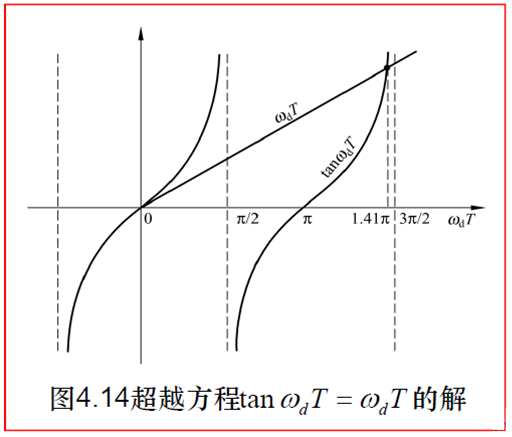
\includegraphics[scale=0.35]{4-14}
\end{columns}
~\\
%\vspace{0.001}
\end{frame}

\begin{frame}[shrink]{一般二元信号波形的检测例题2: 解(续8)}
为了实现简单, 通常采用正交信号, 此时相关系数为0.\\
为了获得与相关系数为$-0.21$时相同的错误概率,需要改变发送信号的能量, 即
\begin{align*}
\left.\sqrt{\frac{E_s}{N_0}(1-\rho)}\right|_{\rho=-0.21}=\sqrt{\frac{E_s^\prime}{N_0}}\\
E_s^\prime=1.21E_s
\end{align*}
\end{frame}

\section{二元信号波形的检测归纳}

\begin{frame}{二元信号波形的检测归纳(1)}
\begin{enumerate}
	\setlength{\itemsep}{.5cm}
	\item \textbf{基本检测方法(正交级数展开法)}
	\begin{itemize}
		\item 首先,利用随机过程的正交级数展开,将随机过程用一组随机变量来表示;
		\item 然后,针对展开得到的随机变量,取前N个展开系数,利用第三章的统计检测方法,构建贝叶斯检测表达式(白高斯噪声条件下,展开系数是不相关的,也是独立的);
		\item 最后,令N趋向于无穷大,求极限,得到波形信号的检测表达式。	
	\end{itemize}
    \item \textbf{充份量统计法}
    \begin{itemize}
    	\item 利用信源发送信号,构建一组特殊的正交函数集,可以利用有限个展开系数构建波形检测表达式。
    \end{itemize}	
\end{enumerate}
\end{frame}

\begin{frame}{二元信号波形的检测归纳(2)}
\textbf{检测性能与偏移系数有关}
\[
d^2\mathop{=}^{def}\frac{\left(E[l|H_1]-E[l|H_0]\right)^2}{Var[l|H_0]}
\]
\textbf{简单二元信号}
\[d^2=\frac{2E_s}{N_0}\]
\textbf{一般二元信号}
\[d^2=\frac{2}{N_0}\left(E_1+E_0-2\rho\sqrt{E_1E_0}\right) \]
\end{frame}

\begin{frame}{二元信号波形的检测归纳(3)}
\begin{itemize}
	\setlength{\itemsep}{.5cm}
	\item 对简单二元信号,只要保持信号$s(t)$的能量不变,信号波形可以\textbf{任意}设计,检测性能不发生变化。
	\item 在高斯白噪声条件下,对于确知一般二元信号的波形检测,当两个信号设计成\textbf{互反信号}时,可在信号能量给定的约束下获得最好的检测性能。	
\end{itemize}
\end{frame}

\begin{frame}[shrink]{二元信号波形的检测归纳(4)}
一般二元信号波形检测的判决表达式为
\begin{align*}
l[x(t)]\mathop{=}^{def}\left(\sqrt{E_1}-\rho\sqrt{E_0}\right)x_1-\left(\sqrt{(1-\rho^2)E_0}\right)x_2\mathop{\gtrless}_{H_0}^{H_1}\frac{N_0}{2}\ln\eta+\frac{1}{2}(E_1-E_0)
\end{align*}
当判决表达式去等号时,
\begin{align*}
\left(\sqrt{E_1}-\rho\sqrt{E_0}\right)x_1-\left(\sqrt{(1-\rho^2)E_0}\right)x_2\mathop{=}^{def}\gamma
\end{align*}
\begin{columns}%[T]
	\column{0.4\textwidth}
	由该方程确定的直线,是判定假设$H_0$成立还是判决假设$H_1$成立的分界线。
	\column{0.5\textwidth}
	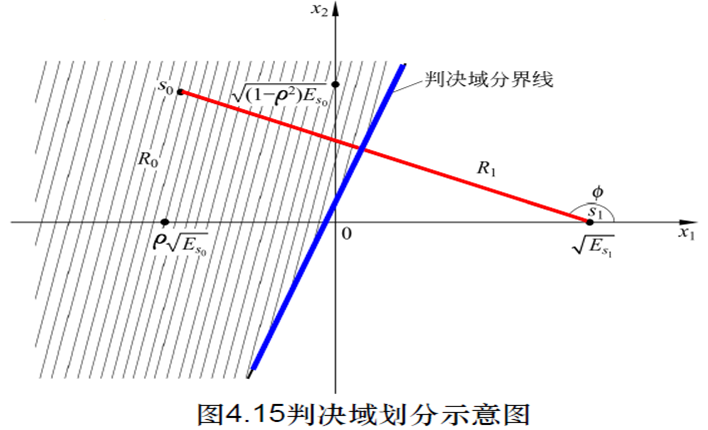
\includegraphics[scale=0.4]{4-15}
\end{columns}
~\\
\end{frame}

\begin{frame}[shrink]{二元信号波形的检测归纳(5)}
\begin{align*}
x_2=\frac{\sqrt{E_1}-\rho\sqrt{E_0}}{\sqrt{(1-\rho^2)E_0}}x_1-\frac{\gamma}{\sqrt{(1-\rho^2)E_0}}
\end{align*}
直线的斜率为:
\[k_x=\frac{\sqrt{E_1}-\rho\sqrt{E_0}}{\sqrt{(1-\rho^2)E_0}} \]
信号$s_0(t)$与$s_1(t)$差向量为:
\begin{align*}
s_0(t)-s_1(t)&=\rho\sqrt{E_0}f_1(t)+\sqrt{(1-\rho^2)E_0}f_2(t)-\sqrt{E_1}f_1(t)\\
&=\left(\rho\sqrt{E_0}-\sqrt{E_1}\right)f_1(t)+\sqrt{(1-\rho^2)E_0}f_2(t)
\end{align*}
\begin{columns}%[T]
\column{0.4\textwidth}
差向量曲线的斜率为:
\begin{align*}
&k_s=\tan\phi=\frac{\sqrt{(1-\rho^2)E_0}}{\rho\sqrt{E_0}-\sqrt{E_1}}\\
&k_xk_s=-1
\end{align*}
判决区域分界线是垂直于信号间连线的一条直线。
\column{0.5\textwidth}
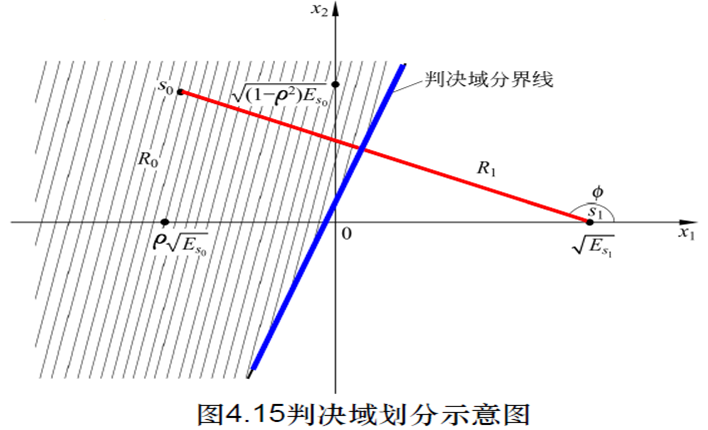
\includegraphics[scale=0.4]{4-15}
\end{columns}
~\\
\end{frame}

\begin{frame}[shrink]{二元信号波形的检测归纳(6)}
如果二元信号假设的先验概率相等,并采用最小平均错误概率准则,则判决域的分界线应满足如下方程:
\begin{align*}
&\exp\left(
\frac{1}{N_0}\left[\left(x_1-\rho\sqrt{E_0}\right)^2+
\left(x_2-\sqrt{(1-\rho^2)E_0}\right)^2\right]-
\frac{1}{N_0}\left[\left(x_1-\sqrt{E_1}\right)^2+x_2^2\right]
\right)\mathop{\gtrless}_{H_0}^{H_1}\eta=1\\
&\left(x_1-\rho\sqrt{E_0}\right)^2+
\left(x_2-\sqrt{(1-\rho^2)E_0}\right)^2=\left(x_1-\sqrt{E_1}\right)^2+x_2^2
\end{align*}
即判决域的分界线是信号$s_0(t)$与信号$s_1(t)$连线的垂直平分线。
\begin{columns}%[T]
	\column{0.4\textwidth}
	如果进一步假设两个信号能量相等,则有:
	\begin{align*}
	\sqrt{1-\rho}x_1=\sqrt{1+\rho}x_2
	\end{align*}
	判决域的分界线是信号$s_0(t)$与信号$s_1(t)$连线的垂直平分线,并通过原点。
	\column{0.5\textwidth}
	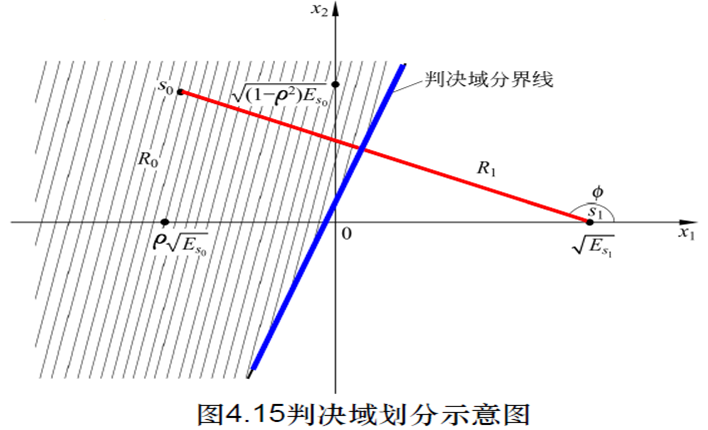
\includegraphics[scale=0.4]{4-15}
\end{columns}
~\\
\end{frame}



